\documentclass[11pt]{article}
\usepackage[utf8]{inputenc}
\usepackage[T5]{fontenc}
\usepackage[margin=1in]{geometry}
\usepackage{float}
\usepackage{xurl}
\usepackage{graphicx}
\usepackage{tikz}
\usepackage{listings}
\usepackage{indentfirst}
\usepackage{amsmath}
\usepackage{booktabs}
\usetikzlibrary{arrows.meta, positioning}

\begin{document}

\begin{center}

{\Large \textbf{UNIVERSITY OF SCIENCE AND TECHNOLOGY OF HANOI}}\\
\vspace{0.3cm}
----------------------o0o----------------------\\

\vspace{4cm}

{\large
\centerline{2540027 - Nguyễn Xuân Vinh}
}

\vspace{4cm}

{\Huge \textbf{BC3.04a Advanced Programming for HPC}}\\
\vspace{0.5cm}
Lecturer: Dr. Trần Giang Sơn

\vspace{4cm}

{\Large \textbf{REPORT LABWORK 4}}\\

\vspace{0.5cm}

{\large
Subjects: Threads
}

\vspace{4cm}
\today
\end{center}

\newpage

\newpage

\tableofcontents

\newpage

\section{Introduction}

The labwork improves the RGB-to-grayscale image converter from Labwork 3.
The previous implementation used a one-dimensional CUDA grid, where the
image was flattened and each CUDA thread processed one pixel.

In the labwork, the image is processed using a two-dimensional CUDA grid
and two-dimensional thread blocks. Different 2D block sizes are tested to
study their effect on GPU execution time and speedup.

The CPU implementation is used as the baseline for calculating speedup.

\section{Image and CPU Implementation}

The input image has the following dimensions:

\begin{itemize}
    \item Width: 1080 pixels
    \item Height: 1920 pixels
    \item Channels: 3 (RGB)
    \item Total pixels: 2,073,600
\end{itemize}

The grayscale value of each pixel is calculated using the standard weighted
RGB formula:

\[
Gray = 0.299R + 0.587G + 0.114B
\]

The CPU implementation processes the pixels sequentially using a
\texttt{for} loop.

The measured CPU execution time was:

\[
T_{CPU} = 1.865874\text{ s}
\]

\section{Improvement from Labwork 3}

In Labwork 3, the image was flattened into a one-dimensional array.
The CUDA kernel used:

\begin{verbatim}
i = cuda.grid(1)
\end{verbatim}

Therefore, each CUDA thread was responsible for one flattened pixel.

For Labwork 4, the original two-dimensional image structure is preserved.
The CUDA kernel uses:

\begin{verbatim}
x, y = cuda.grid(2)
\end{verbatim}

The pixel at position $(x,y)$ is then accessed directly as:

\begin{verbatim}
rgb_image[y, x, channel]
\end{verbatim}

Thus, the CUDA thread organization matches the spatial structure of the
image more naturally.

The 2D kernel also checks the image boundaries before accessing a pixel:

\begin{verbatim}
if x < width and y < height:
\end{verbatim}

This prevents threads outside the image dimensions from accessing invalid
memory.

\section{1D CUDA Performance}

The original Labwork 3 implementation used 256 threads per block and
8100 blocks.

The measured results were:

\begin{table}[H]
    \centering
    \caption{CPU and 1D CUDA performance}
    \begin{tabular}{lcc}
        \toprule
        Implementation & Time (s) & Speedup \\
        \midrule
        CPU & 1.865874 & 1.00$\times$ \\
        CUDA 1D & 0.000665 & 2804.03$\times$ \\
        \bottomrule
    \end{tabular}
\end{table}

The speedup is calculated as:

\[
Speedup = \frac{T_{CPU}}{T_{GPU}}
\]

Therefore:

\[
Speedup_{1D}
=
\frac{1.865874}{0.000665}
\approx 2804.03
\]

\section{2D Block Size Experiment}

Several two-dimensional block configurations were tested. Each
configuration was executed multiple times and the average execution time
was recorded.

\begin{table}[H]
    \centering
    \caption{Performance of different 2D block sizes}
    \begin{tabular}{c c c c}
        \toprule
        Block Size & Threads/Block & Time (s) & Speedup \\
        \midrule
        $4\times4$   & 16  & 0.000790 & 2361.94$\times$ \\
        $8\times8$   & 64  & 0.000416 & 4482.27$\times$ \\
        $16\times16$ & 256 & 0.000399 & 4670.59$\times$ \\
        $32\times8$  & 256 & 0.000399 & 4679.53$\times$ \\
        $8\times32$  & 256 & 0.000400 & 4662.24$\times$ \\
        $32\times16$ & 512 & 0.000401 & 4657.25$\times$ \\
        \bottomrule
    \end{tabular}
\end{table}

The following graph shows the relationship between 2D block size and
speedup.

\begin{figure}[H]
    \centering
    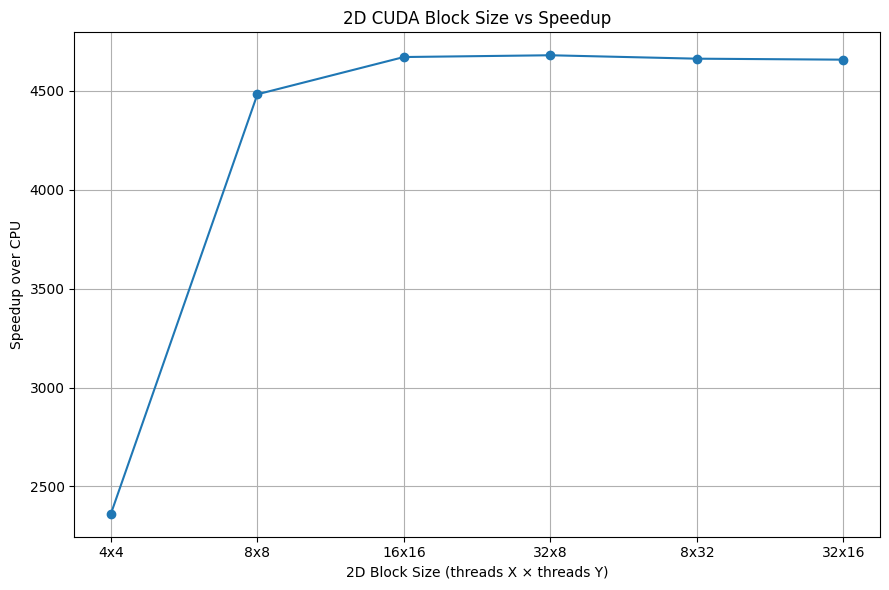
\includegraphics[width=0.85\textwidth]
    {block_size_2d_vs_speedup.png}
    \caption{2D CUDA block size versus speedup}
    \label{fig:block-speedup}
\end{figure}

Among the tested configurations, the $8\times32$ block produced the lowest
measured execution time:

\[
T_{2D} = 0.000399\text{ s}
\]

and the highest measured speedup:

\[
Speedup_{2D} = 4679.53\times
\]

The result should be understood as the best measured configuration among
the tested block sizes, rather than a universally optimal CUDA block size.

\section{Comparison Between 1D and 2D CUDA}

The best measured 2D configuration was compared with the original 1D
implementation.

\begin{table}[H]
    \centering
    \caption{Comparison between 1D and 2D CUDA}
    \begin{tabular}{lcc}
        \toprule
        Implementation & GPU Time (s) & Speedup \\
        \midrule
        CUDA 1D & 0.000665 & 2804.03$\times$ \\
        CUDA 2D & 0.000399 & 4679.53$\times$ \\
        \bottomrule
    \end{tabular}
\end{table}

The measured execution-time ratio between the two GPU implementations is:

\[
\frac{0.000665}{0.000399}
\approx 1.67
\]

Therefore, in this experiment, the best tested 2D configuration was about
$1.67\times$ faster than the 1D implementation in terms of measured GPU
kernel execution time.

\section{Validation}

The CPU, 1D CUDA, and 2D CUDA implementations produce the same grayscale
image within floating-point tolerance.

The maximum difference between CPU and GPU results was:

\[
2.53544\times10^{-6}
\]

and the mean difference was:

\[
2.53544\times10^{-6}
\]

Both GPU implementations passed the numerical validation using
\texttt{np.allclose()}.

Therefore, the 2D implementation improves the CUDA thread organization
without changing the correctness of the grayscale conversion.

\section{Discussion}

The experiment shows that CUDA block configuration affects GPU execution
time. The $4\times4$ configuration had the lowest number of threads per
block and produced the slowest result among the tested configurations.

Increasing the number of threads per block significantly improved the
execution time. Configurations using 256 threads per block, such as
$16\times16$, $32\times8$, and $8\times32$, achieved similar and better
performance.

The $32\times8$ configuration achieved the lowest measured execution time
in this experiment. However, the differences between several configurations
were very small, so measurement noise and GPU runtime conditions may affect
the exact values.

The timing measures GPU kernel execution after the input data has already
been transferred to the GPU. Therefore, the reported speedups do not
represent the complete image-processing pipeline including host-to-device
and device-to-host memory transfers.

\section{Thread Model Exercises}

\subsection{Exercise 1}

Consider a GPU with the following maximum specifications:

\begin{itemize}
    \item 512 threads per block
    \item 1024 threads per SM
    \item 8 blocks per SM
    \item 32 threads per warp
\end{itemize}

The possible configurations are:

\begin{itemize}
    \item $8\times8 = 64$ threads
    \item $16\times16 = 256$ threads
    \item $32\times32 = 1024$ threads
\end{itemize}

The $32\times32$ configuration is not valid because it requires 1024
threads per block, which exceeds the maximum of 512 threads per block.

Both $8\times8$ and $16\times16$ are valid configurations. The
$16\times16$ configuration provides 256 threads per block, corresponding
to 8 warps:

\[
\frac{256}{32}=8\text{ warps}
\]

Therefore, among the given choices, the best configuration is:

\[
\boxed{16\times16}
\]

\subsection{Exercise 2}

The SM can accommodate a maximum of 1,536 threads and 4 blocks.

For 128 threads per block:

\[
128\times4=512\text{ threads}
\]

For 256 threads per block:

\[
256\times4=1024\text{ threads}
\]

For 512 threads per block:

\[
512\times3=1536\text{ threads}
\]

For 1024 threads per block, only one block can be scheduled because
the block itself uses 1024 threads:

\[
1024\times1=1024\text{ threads}
\]

Therefore, the configuration that results in the largest number of
threads in the SM is:

\[
\boxed{512\text{ threads/block}}
\]

This allows:

\[
\boxed{1536\text{ threads}}
\]

to be active in the SM.

\subsection{Exercise 3}

The vector contains 2,000 elements, and each thread produces one output.
The block size is 512 threads.

The required number of blocks is:

\[
\left\lceil\frac{2000}{512}\right\rceil=4
\]

Therefore, the total number of threads launched is:

\[
4\times512=2048
\]

Thus, the grid contains:

\[
\boxed{2048\text{ threads}}
\]

Only 2,000 threads are required for the vector elements, so 48 threads
in the last block do not process a valid element. A boundary check such
as \texttt{if i < 2000} is therefore required.

\section{Conclusion}

Labwork 4 successfully improved the previous RGB-to-grayscale CUDA
implementation from a one-dimensional grid to a two-dimensional grid.
Several 2D block configurations were tested and their execution times and
speedups were compared.

The best tested configuration was $32\times8$, with a measured GPU
execution time of approximately $0.000399$ seconds and a speedup of
$4679.53\times$ relative to the CPU implementation. Compared with the
previous 1D CUDA implementation, the measured GPU execution was
approximately $1.67\times$ faster.

The CPU, 1D CUDA, and 2D CUDA results were also numerically validated,
confirming that the performance improvement did not change the correctness
of the grayscale conversion.

\end{document}